\documentclass[10pt,a4paper]{article}
\usepackage[utf8]{inputenc}
\usepackage{amsmath}
\usepackage{amssymb}
\usepackage[margin=1in]{geometry}
\usepackage{setspace}
\usepackage{tikz}
\usepackage{pgfplots}
\usepackage{listings}
\pgfplotsset{compat=1.18}

\title{Methods Questions}
\author{}
\date{}

\begin{document}

\maketitle

\section*{Question 1 [TF]}

\textbf{Question 8} \hfill 7 marks

A random variable $X$ has a probability density function given by

\[
f(x) = \begin{cases}
k\cos^2(x) + k & 0 \leq x \leq \frac{\pi}{2} \\
0 & \text{elsewhere}
\end{cases}
\]

where $k \geq 0$.

\textbf{(a)} Show that $\frac{d}{dx}(x + \sin(x)\cos(x)) = 2\cos^2(x)$.

\vspace{9\baselineskip}

\textbf{(b)} Hence, find the value of $k$. Express your answer in the form $\frac{a-\pi}{b\pi}$.

\vspace{9\baselineskip}

\hrulefill

\section*{Question 2 [TF]}

\textbf{Question 8(d)} \hfill 7 marks

Another random variable $Y$ has probability density function given by

\[
g(x) = \begin{cases}
a\cos^2(x) + c & 0 \leq x \leq \frac{\pi}{2} \\
0 & \text{elsewhere}
\end{cases}
\]

where $a \geq 0$.

Find the maximum value of $a$.

\vspace{9\baselineskip}

\hrulefill

\section*{Question 3 [TA]}

\textbf{Question 19} \hfill 1 mark

If $\cos(a) = b$, where $b < 0$ and $\frac{\pi}{2} < a < \pi$, then the sum of the solutions to $\cos(3x) = b$, where $0 < x < \pi$, is

\begin{enumerate}
    \item[A.] $a$
    \item[B.] $\frac{3a + 2\pi}{3}$
    \item[C.] $a + 2\pi$
    \item[D.] $\frac{2(a + \pi)}{3}$
\end{enumerate}

\vspace{9\baselineskip}

\hrulefill

\section*{Question 4 [TA]}

\textbf{Question 2} \hfill 12 marks

The strength of a signal is modelled by $f(t) = 5 - 3\sin\left(\frac{\pi t}{8}\right)$ where time $t$ is in seconds and $t \geq 0$.

\textbf{(g)} For two distinct times $t_1, t_2 \in (0, 16)$, an observer notes that $f'(t_1) = -f'(t_2)$. $t_2$ can be expressed as

\[
t_2 = \begin{cases}
c_1 - t_1 & 0 < t_1 < 8 \text{ and } 0 < t_2 < 8 \\
c_2 - t_1 & 8 < t_1 < 16 \text{ and } 8 < t_2 < 16
\end{cases}
\]

Find the values of $c_1$ and $c_2$.

\vspace{9\baselineskip}

\hrulefill

\section*{Question 5 [TA]}

\textbf{Question 4} \hfill 14 marks

The durations (in seconds) for which ads are viewed on a YouTube channel follow the probability density function:

\[
f(x) = \begin{cases}
\frac{16}{15(x-5)^2} & 6 \leq x \leq 21 \\
0 & \text{elsewhere}
\end{cases}
\]

\textbf{(a)} Find the probability that an ad is viewed for more than 10 seconds.

\vspace{9\baselineskip}

\textbf{(c)} Another probability distribution function is given by

\[
g(x) = \begin{cases}
af(x) - b & 6 \leq x \leq 21 \\
0 & \text{elsewhere}
\end{cases}
\]

where $a, b > 0$. Find the maximum value of $b$ and the corresponding value of $a$.

\vspace{9\baselineskip}

\hrulefill

\section*{Question 6 [TA]}

\textbf{Question 5}

Let $g : (-3,\infty) \to \mathbb{R}$, $g(x) = -\log_e(2x + 6)$.

$h : [0,\infty) \to \mathbb{R}$, $h(x) = a\cos(x)$, where $a \neq 0$.

\textbf{(e)} Find the values of $a$ for which the graphs of $h$ and $g$ do not intersect. Give any non-exact values correct to two decimal places.

\vspace{9\baselineskip}

\hrulefill

\section*{Question 7 [TA]}

\textbf{Question 10}

A 99\% confidence interval for a population proportion is equal to $(a,b)$, then a 95\% confidence interval for the population proportion is closest to

\begin{enumerate}
    \item[A.] $(0.88a + 0.12b, 0.12a + 0.88b)$
    \item[B.] $(0.88a - 0.12b, 0.12a + 0.88b)$
    \item[C.] $(1.31a, 1.31b)$
    \item[D.] $(0.76a, 0.76b)$
\end{enumerate}

\vspace{9\baselineskip}

\hrulefill

\section*{Question 8 [TA]}

\textbf{Question 17}

Several students were considering the following simultaneous equations

\begin{align*}
3x - 2y + z &= 1\\
-x + y - z &= 2
\end{align*}

Allan stated that the general solution could be expressed as
\[
x = k, \quad y = 2k - 3, \quad z = k - 5 \quad \text{for } k \in R.
\]

Ben stated that the general solution could be expressed as
\[
x = \frac{k+3}{2}, \quad y = k, \quad z = \frac{k-7}{2} \quad \text{for } k \in R.
\]

Colin stated that the general solution could be expressed as
\[
x = k + 5, \quad y = 2k + 7, \quad z = k \quad \text{for } k \in R.
\]

Then

\begin{enumerate}
    \item[A.] Only Allan is correct.
    \item[B.] Only Ben is correct
    \item[C.] Only Colin is correct
    \item[D.] All of Allan, Ben and Colin are correct.
\end{enumerate}

\vspace{9\baselineskip}

\hrulefill

\section*{Question 9 [TA]}

\textbf{Question 18}

Newton's method is used to solve the equation $f(x) = 0$.

Newton's method can sometimes fail to find the root of the equation $f(x) = 0$.

All of the functions below have a root close to $x = 1$, with a starting value of $x_0 = 2$. Newton's method will succeed for which one of the following functions?

\begin{enumerate}
    \item[A.] $f(x) = \sqrt{3x^2 - 7x + 2}$
    \item[B.] $f(x) = 3x^3 - 13x^2 + 16x - 4$
    \item[C.] $f(x) = (3x - 1)\log_e(x - 2)$
    \item[D.] $f(x) = (3x - 1)e^{x-2}$
\end{enumerate}

\vspace{9\baselineskip}

\hrulefill

\section*{Question 10 [TF]}

\textbf{Question 3} \hfill 3 marks

Find the values of $a$ and $b$ for which the simultaneous linear equations,

\begin{align*}
2ax - 2by &= 5\\
(1-3b)x + 12y &= 2 - 4b
\end{align*}

have an infinite number of solutions.

\vspace{9\baselineskip}

\hrulefill

\section*{Question 11 [TF]}

\textbf{Question b} \hfill 3 marks

Consider the functions $f : [0,2\pi] \to R$, $f(x) = 2\sin^2(2x)$ and $g : [0,2\pi] \to R$, $g(x) = 1 - \cos(2x)$, on the axes below, sketch the graphs of the functions $y = f(x)$ and $y = g(x)$ [...]

\vspace{9\baselineskip}

\hrulefill

\section*{Question 12 [TF]}

\textbf{Question 2} \hfill 6 marks

Consider line $l_1$ with equation $y = 2x - 3$ and line $l_2$ that is perpendicular to $l_1$ and passes through its $y$-intercept.

\textbf{(a)} Show that the equation of $l_2$ is $y = -\frac{1}{2}x - 3$.

\vspace{9\baselineskip}

\textbf{(b)} Another line $l_3$ has the equation $y = mx + c$, where $m,c \in \mathbb{R}$.

\textbf{i.} If the simultaneous equations $l_1$, $l_2$ and $l_3$ have a unique solution, find the possible values of $m$ and $c$.

\vspace{9\baselineskip}

\textbf{ii.} Find the positive value of $m$ for which $l_3$ passes through the point $(3,3)$ and encloses an isosceles triangle with $l_1$ and $l_2$.

\vspace{9\baselineskip}

\hrulefill

\section*{Question 13 [TF]}

\textbf{Part (c)} \hfill 3 marks

The graph of $f : \left[0, \frac{\pi}{2}\right] \to \mathbb{R}$, $f(x) = \sqrt{\sin(2x)}$ is shown below.

On the same set of axes, sketch the graph of the derivative function $f'$. Label any asymptotes with their equations and any intercepts with their coordinates. You do not need to label any point [...]

\vspace{9\baselineskip}

\hrulefill

\section*{Question 14 [TF]}

\textbf{Part (e)} \hfill 3 marks

The function $g(x) = a\sqrt{b - (x - c)^2}$ has the same domain and range as $f$. Find the values of $a$, $b$ and $c$.

\vspace{9\baselineskip}

\hrulefill

\section*{Question 15 [TA]}

\textbf{Question 2}

Let $g : [150,210] \to \mathbb{R}$, $g(x) = \frac{\pi}{120}\sin\left(\frac{\pi}{60}(x - 30)\right)$.

In a farm, the masses of apples in grams are represented by a random variable $X$ with the probability density function

\[
f(x) = \begin{cases}
g(x) & 150 \leq x \leq 210\\
0 & \text{elsewhere}
\end{cases}
\]

\textbf{(i)} If $\text{Pr}(b - c < X < b + c) = 0.9$, where $b - c \geq 150$ and $b + c \leq 210$, find the possible values of $b$, correct to one decimal place.

\vspace{9\baselineskip}

\hrulefill

\section*{Question 16 [TA]}

\textbf{Question 4} \hfill 2 marks

In a cattle ranch, an agriculturist monitors two identical cows, A and B, over 20 months to study the effects of food deprivation. Cow A receives a normal diet throughout, while Cow B is placed on a restricted diet for the first 10 months and then resumes a normal diet. The weight gains of the cows over time are plotted below. Both cows have gained 400 kg after 20 months.

\begin{center}
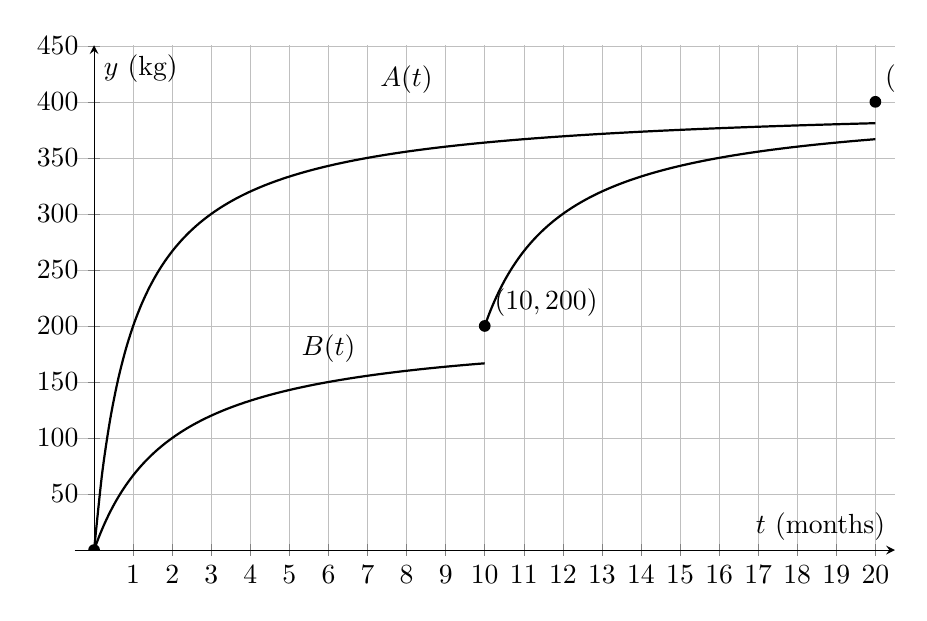
\begin{tikzpicture}
\begin{axis}[
 width=12cm,
 height=8cm,
 xlabel={$t$ (months)},
 ylabel={$y$ (kg)},
 xmin=0, xmax=20,
 ymin=0, ymax=450,
 xtick={0,1,2,3,4,5,6,7,8,9,10,11,12,13,14,15,16,17,18,19,20},
 ytick={0,50,100,150,200,250,300,350,400,450},
 grid=both,
 grid style={line width=.1pt, draw=gray!30},
 major grid style={line width=.2pt,draw=gray!50},
 axis lines=middle,
 enlargelimits={abs=0.5},
]

% Curve A(t)
\addplot[
 domain=0:20,
 samples=100,
 smooth,
 thick,
 black,
] {400 - 400/(x+1)};
\node at (axis cs:8,420) {$A(t)$};
\node[circle,fill,inner sep=1.5pt] at (axis cs:20,400) {};
\node[above right] at (axis cs:20,400) {$(20,400)$};

% Curve B(t) - first part (0 to 10)
\addplot[
 domain=0:10,
 samples=100,
 smooth,
 thick,
 black,
] {200 - 200/(0.5*x+1)};

% Curve B(t) - second part (10 to 20)
\addplot[
 domain=10:20,
 samples=100,
 smooth,
 thick,
 black,
] {200 + 200 - 200/(0.5*(x-10)+1)};
\node at (axis cs:6,180) {$B(t)$};
\node[circle,fill,inner sep=1.5pt] at (axis cs:10,200) {};
\node[above right] at (axis cs:10,200) {$(10,200)$};

% Origin point
\node[circle,fill,inner sep=1.5pt] at (axis cs:0,0) {};
\node[below left] at (axis cs:0,0) {$(0,0)$};

\end{axis}
\end{tikzpicture}
\end{center}

Cow A's weight gain, $A(t)$ in kg after $t$ months is modelled by

\[
A : [0,20] \to \mathbb{R}, \quad A(t) = p - \frac{p}{t + q}
\]

where $p$ and $q$ are positive constants.

Cow B's weight gain, $B(t)$ in kg after $t$ months is modelled by

\[
B(t) = \begin{cases}
B_1(t) & 0 \leq t \leq 10\\
B_2(t) & 10 < t \leq 20
\end{cases}
\]

where $B_1(t)$ and $B_2(t)$ are linear transformations of the graph of $A(t)$. The graphs of $B_1(t)$ and $B_2(t)$ are joined at the point $(10,200)$.

\textbf{(a)} Describe a sequence of transformations that maps the graph of $A(t)$ to the graph of $B_2(t)$.

\vspace{9\baselineskip}

\hrulefill

\section*{Question 17 [TA]}

\textbf{Question 7} \hfill 1 mark

A fair six-sided die is rolled until a '6' appears, and the number of rolls is noted. The probability that a '6' appears in at most $n$ rolls is

\begin{enumerate}
    \item[A.] $\left(\frac{5}{6}\right)^n$
    \item[B.] $1 - \left(\frac{5}{6}\right)^n$
    \item[C.] $\frac{1}{6}\left(\frac{5}{6}\right)^n$
    \item[D.] $1 - \frac{1}{6}\left(\frac{5}{6}\right)^n$
\end{enumerate}

\vspace{9\baselineskip}

\hrulefill

\section*{Question 18 [TA]}

\textbf{Question 12} \hfill 1 mark

A pharmaceutical company is running two independent clinical trials -- one in Sydney and another in Melbourne. Let $S$ be the event that the Sydney trial is successful and $M$ be the event that the Melbourne trial is successful.

Given that at least one of the two trials is successful, what is the probability that only the Melbourne trial is successful, correct to four decimal places?

\begin{enumerate}
    \item[A.] 0.1080
    \item[B.] 0.2045
    \item[C.] 0.3061
    \item[D.] 0.4286
\end{enumerate}

\vspace{9\baselineskip}

\hrulefill

\section*{Question 19 [TF]}

\textbf{Question 8}

\textbf{(a)} Consider the functions $f_1(x) = 2\sin^2(x)$ and $f_2(x) = \cos^2(x)$, where $x \in \mathbb{R}$.

\textbf{i.} State the range of $f_1$.

\vspace{9\baselineskip}

\textbf{ii.} If the $x$-coordinates of the points of intersection of $y = f_1(x)$ and $y = f_2(x)$ satisfy the equation $\tan(x) = k$, find all possible values of $k$.

\vspace{9\baselineskip}

\hrulefill

\section*{Question 20 [TF]}

\textbf{Question 8}

\textbf{ii.} Consider the function $g^* : [0,k] \to \mathbb{R}$, $g^*(x) = \sin(2x^2)$, where $k > 0$. Find all values of $k$ for which the range of $g^*$ is $[-1,1]$.

\vspace{9\baselineskip}

\hrulefill

\section*{Question 21 [TA]}

\textbf{Question 8}

\textbf{(d)} Let $W$ be a random variable representing the density (in tonnes per cubic metre) of concrete cylinders manufactured by a construction company. Suppose its probability density function is given by

\[
w(x) = \begin{cases}
-kx^2 + \left(\frac{38k + 6}{15}\right)x & 2 \leq x \leq 3\\
0 & \text{elsewhere}
\end{cases}
\]

If $\text{Pr}(W > 2.5) = 0.40$, find the values $k$ can take.

\vspace{9\baselineskip}

\hrulefill

\section*{Question 22 [TA]}

\textbf{Question 2} \hfill 1 mark

If $h'(x) = e^{-\frac{1}{4}}$ and $h(1) = 4$, the value of $h(2)$ is closest to

\begin{enumerate}
    \item[A.] 4.6533
    \item[B.] 4.5048
    \item[C.] 6.0201
    \item[D.] 3.9224
\end{enumerate}

\vspace{9\baselineskip}

\hrulefill

\section*{Question 23 [TF]}

\textbf{Part (d)} \hfill 3 marks

Find the real value(s) of $k$ for which the graph of $y = \tan(kx) - 1$ has exactly three $x$-intercepts in $x \in \left[0, \frac{5\pi}{4}\right]$.

\vspace{9\baselineskip}

\hrulefill

\section*{Question 24 [TA]}

\textbf{Question 3} \hfill 17 marks

An athlete training for a triathlon is located at point $O(0,0)$ on the shore of a circular lake of diameter 4 kilometres. To reach the opposite point $Q(4,0)$, the athlete runs around the shore clockwise to point $P$ at a speed of 12 km/h, then swims the remaining distance, if any, to point $Q$ at 6 km/h. Let $\theta = \angle OCP$, where $C$ is the centre of the circle.

\begin{center}
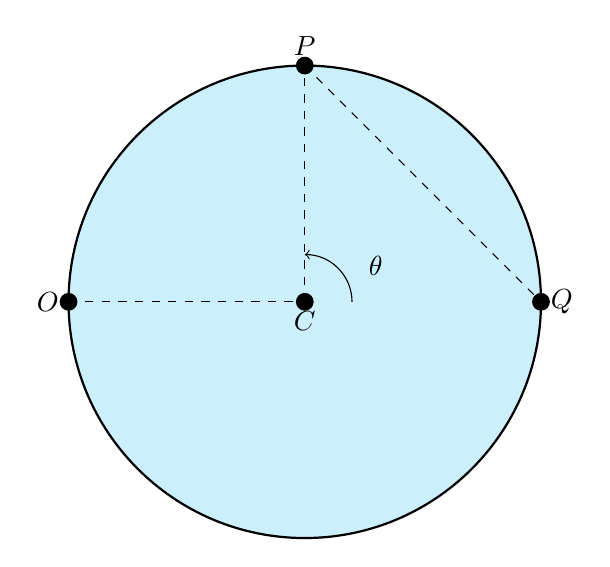
\begin{tikzpicture}[scale=1.5]
    % Draw the circle with light blue fill
    \fill[cyan!20] (2,0) circle (2cm);
    \draw[thick] (2,0) circle (2cm);
    
    % Draw points
    \filldraw[black] (0,0) circle (2pt) node[left] {$O$};
    \filldraw[black] (2,0) circle (2pt) node[below] {$C$};
    \filldraw[black] (4,0) circle (2pt) node[right] {$Q$};
    \filldraw[black] (2,2) circle (2pt) node[above] {$P$};
    
    % Draw dashed lines
    \draw[dashed] (0,0) -- (2,0);
    \draw[dashed] (2,0) -- (2,2);
    \draw[dashed] (2,2) -- (4,0);
    
    % Draw angle theta
    \draw[->] (2.4,0) arc (0:90:0.4);
    \node at (2.6,0.3) {$\theta$};
\end{tikzpicture}
\end{center}

\textbf{(a)} Express the coordinates of $P$ in terms of $\theta$.

\textit{Solution: The centre is at $C(2,0)$. The coordinates of $P$ are $(2 - 2\cos(\theta), 2\sin(\theta))$.}

\vspace{9\baselineskip}

Let $\theta = \frac{\pi}{2}$. The displacement of the athlete, $s(t)$ kilometres (distance relative to the starting point O) after $t$ hours can be expressed as

\[
s(t) = \begin{cases}
s_1(t) & 0 \leq t \leq t_P\\
s_2(t - t_P) & t_P < t \leq t_Q
\end{cases}
\]

where $t_P$ and $t_Q$ are the times taken to reach points $P$ and $Q$, respectively.

\textbf{(e)} Find the rule of $s_1(t)$ in the form $\sqrt{k - m\cos(nx)}$, where $k, m, n \in \mathbb{Z}^+$.

\vspace{9\baselineskip}

\textbf{(f)} Find the rule of $s_2(t - t_P)$. Is the rate of change of the displacement constant for $t_P < t \leq t_Q$?

\vspace{9\baselineskip}

\textbf{(g)} Find the smallest possible values of $a$ and $b$.

The swimming speed, $X$ km/h, of male athletes in the triathlon follows the probability distribution

\[
f(x) = \begin{cases}
\frac{a}{2}\sin(a(x - b)) & 5 \leq x \leq 9\\
0 & \text{elsewhere}
\end{cases}
\]

where $a, b \in \mathbb{R}^+$. The graph of $f(x)$ has $x$-intercepts at $x = 5$ and $x = 9$.

\vspace{9\baselineskip}

\textbf{(h)} The probability distribution for the swimming speed of female athletes ranges from 6 km/h to 8.5 km/h and can be obtained from a sequence of transformations on the graph of $f(x)$.

Describe a sequence of two dilations and one translation to achieve the above transformation.

\vspace{9\baselineskip}

\hrulefill

\section*{Question 25 [TA]}

\textbf{Question 20} \hfill 1 mark

The algorithm below simulates rolling two dice and calculates the probability of having a sum of at least 5 but no more than 10.

\begin{center}
\begin{tabular}{l}
\texttt{count} $\leftarrow$ 0 \\
\texttt{total} $\leftarrow$ 0 \\
\textbf{for} \texttt{i} \textbf{from} 1 \textbf{to} 6 \\
\quad \textbf{for} \texttt{j} \textbf{from} 1 \textbf{to} 6 \\
\quad \quad \underline{\hspace{8cm}} \\
\quad \quad \underline{\hspace{8cm}} \\
\quad \quad \underline{\hspace{8cm}} \\
\quad \quad \underline{\hspace{8cm}} \\
\quad \textbf{end for} \\
\textbf{end for} \\
\textbf{print} $\frac{\texttt{count}}{\texttt{total}}$
\end{tabular}
\end{center}

Which of the following could be the missing lines?

\begin{enumerate}
    \item[A.] 
    \begin{tabular}[t]{l}
    \textbf{if} $5 \leq i+j \leq 10$ \textbf{then} \\
    \quad \texttt{count} $\leftarrow$ \texttt{count} + 1 \\
    \quad \texttt{total} $\leftarrow$ \texttt{total} + 1 \\
    \textbf{end if}
    \end{tabular}
    
    \item[C.] 
    \begin{tabular}[t]{l}
    \textbf{while} $5 \leq i+j \leq 10$ \\
    \quad \texttt{count} $\leftarrow$ \texttt{count} + 1 \\
    \quad \texttt{total} $\leftarrow$ \texttt{total} + 1 \\
    \textbf{end while}
    \end{tabular}
    
    \item[B.] 
    \begin{tabular}[t]{l}
    \texttt{total} $\leftarrow$ \texttt{total} + 1 \\
    \textbf{if} $5 \leq i+j \leq 10$ \textbf{then} \\
    \quad \texttt{count} $\leftarrow$ \texttt{count} + 1 \\
    \textbf{end if}
    \end{tabular}
    
    \item[D.] 
    \begin{tabular}[t]{l}
    \texttt{total} $\leftarrow$ \texttt{total} + 1 \\
    \textbf{while} $5 \leq i+j \leq 10$ \\
    \quad \texttt{count} $\leftarrow$ \texttt{count} + 1 \\
    \textbf{end while}
    \end{tabular}
\end{enumerate}

\vspace{9\baselineskip}

\hrulefill

\section*{Question 26 [TA]}

\textbf{Part (f)}

Part of the graph of $y = f(x)$ is shown below. The line $y = c$ intersects the curve at two points in the first quadrant.

\begin{center}
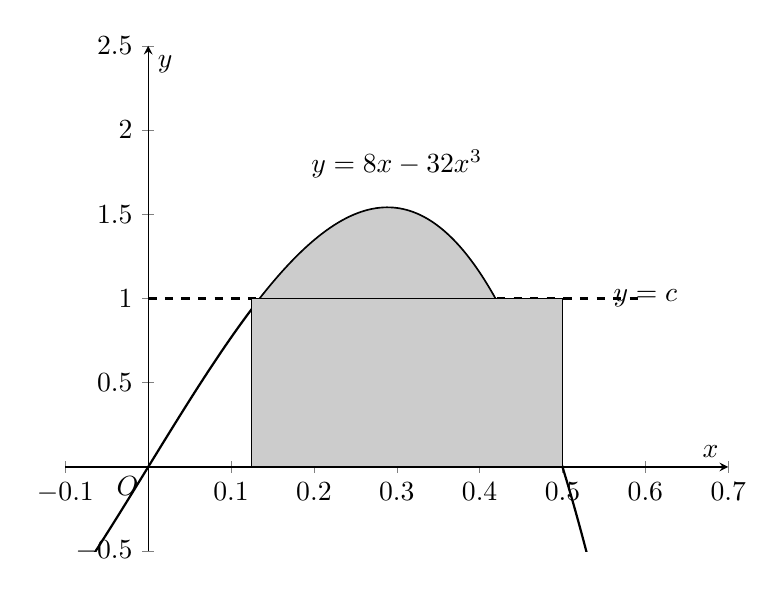
\begin{tikzpicture}
\begin{axis}[
 width=10cm,
 height=8cm,
 xlabel={$x$},
 ylabel={$y$},
 xmin=-0.1, xmax=0.7,
 ymin=-0.5, ymax=2.5,
 axis lines=middle,
 samples=100,
 domain=-0.1:0.7,
]

% Draw the curve y = 8x - 32x^3
\addplot[thick, black, smooth] {8*x - 32*x^3};
\node at (axis cs:0.3,1.8) {$y = 8x - 32x^3$};

% Draw horizontal line y = c
\addplot[thick, dashed] coordinates {(0,1) (0.6,1)};
\node at (axis cs:0.55,1) [right] {$y = c$};

% Shaded regions
\addplot[fill=gray!40, domain=0.125:0.5] {8*x - 32*x^3} \closedcycle;
\addplot[fill=gray!40] coordinates {(0.125,1) (0.5,1) (0.5,0) (0.125,0)} \closedcycle;

% Mark origin
\node at (axis cs:0,0) [below left] {$O$};

\end{axis}
\end{tikzpicture}
\end{center}

\textbf{i.} Find the total area of the shaded regions when $c = 1$. Give your answer correct to three decimal places. \hfill [3 marks]

\vspace{9\baselineskip}

\hrulefill

\section*{Question 27 [TA]}

\textbf{Part (ii)}

Find the value of $c$ such that the areas of the shaded regions are equal.

\vspace{9\baselineskip}

\hrulefill

\section*{Question 28 [TA]}

\textbf{Part (h)} \hfill 2 marks

In general, the concentration of a drug in the bloodstream can be modelled by $d(t) = a(1 - e^{-kt}) - mt$, where $a$, $k$ and $m$ are positive constants. State a restriction on $k$ (in terms of $a$ and $m$) for this model to be valid.

\vspace{9\baselineskip}

\hrulefill

\section*{Question 29 [TF]}

\textbf{Part (d)} \hfill 2 marks

To investigate and ameliorate this decline, VCAA experiments with different course difficulties with different values of $p$, which denotes the probability that any student achieves raw study score over 40. $p_1$ and $p_2$ are two particular values that VCAA considers. Let $P^*$ represent the proportion of students under this new difficulty that achieve a raw study score above 40.

The value of $\sigma(P^*)$ when $p = p_2$ is twice as large as the value of $\sigma(P^*)$ when $p = p_1$. What is the maximum value of $p_1$, given that $p_i < \frac{1}{2}$?

\vspace{9\baselineskip}

\hrulefill

\section*{Question 30 [TF]}

\textbf{Question 8} \hfill $(1+3)+4 = 8$ marks

Consider $f : (0,\infty) \to \mathbb{R}$, $f(x) = \frac{1}{x^2} - 1$.

\textbf{a. i.} Let $g(x) = f(x) + f'(x) + c$, where $c \in \mathbb{R}$. Find the rule of $g(x)$. \hfill (1 mark)

\vspace{9\baselineskip}

\textbf{ii.} If the graph of $g(x)$ has one $x$ intercept, what are the possible $x$ values of this intercept? \hfill (3 marks)

\vspace{9\baselineskip}

\hrulefill

\section*{Question 31 [TA]}

\textbf{Part (d)}

Let $g : \mathbb{R} \to \mathbb{R}$, $g(x) = (1-x)(x+2)$ and $h : \mathbb{R} \to \mathbb{R}$, $h(x) = x - 3k$, where $k < -1$. The graphs of $g$ and $h$ are shown below.

\begin{center}
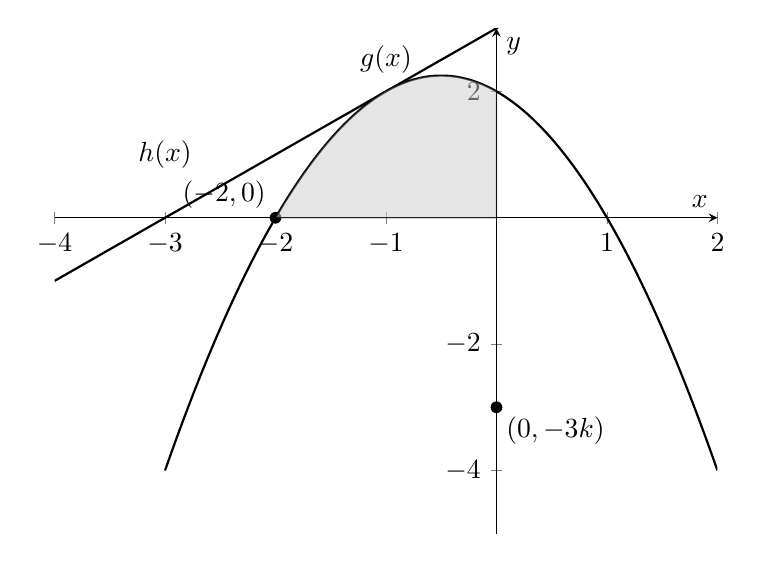
\begin{tikzpicture}
\begin{axis}[
 width=10cm,
 height=8cm,
 xlabel={$x$},
 ylabel={$y$},
 xmin=-4, xmax=2,
 ymin=-5, ymax=3,
 axis lines=middle,
 samples=100,
]

% Parabola g(x) = (1-x)(x+2)
\addplot[thick, black, smooth, domain=-3:2] {(1-x)*(x+2)};
\node at (axis cs:-1,2.5) {$g(x)$};

% Line h(x) = x - 3k (assuming k = -1 for visualization)
\addplot[thick, black, domain=-4:2] {x + 3};
\node at (axis cs:-3,1) {$h(x)$};

% Point labels
\node[circle,fill,inner sep=1.5pt] at (axis cs:0,-3) {};
\node at (axis cs:0,-3) [below right] {$(0,-3k)$};
\node[circle,fill,inner sep=1.5pt] at (axis cs:-2,0) {};
\node at (axis cs:-2,0) [above left] {$(-2,0)$};
\node[circle,fill,inner sep=1.5pt] at (axis cs:3,0) {};
\node at (axis cs:3,0) [above right] {$(3k,0)$};

% Shaded region
\addplot[fill=gray!40, domain=-2:0, opacity=0.5] {(1-x)*(x+2)} \closedcycle;

\end{axis}
\end{tikzpicture}
\end{center}

In the figure, let $A_1$ be the area bounded by the graphs of $g$, $h$ and the coordinate axes in the second quadrant.

\textbf{i.} Find $A_1$ in terms of $k$. \hfill [2 marks]

\vspace{9\baselineskip}

\textbf{iii.} If the shortest distance between a point on $g$ and $h$ is 1 unit, find the value of $k$. \hfill [3 marks]

\vspace{9\baselineskip}

\hrulefill

\section*{Question 32 [TA]}

\textbf{Part (d)}

Let $l$ be the line with equation $y = -\frac{4x}{3}$ and $l_p$ be the line tangent to $f$ at $x = p$.

\textbf{i.} Find one of the two possible equations of $l_p$ if it is perpendicular to $l$. Give your answer in the form $y = mx + b$, where $m$ and $b$ are correct to two decimal places. \hfill [2 marks]

\vspace{9\baselineskip}

\textbf{ii.} As $p \to 2$, the acute angle between $l$ and $l_p$ approaches $\theta$. Find $\tan(\theta)$.

\vspace{9\baselineskip}

\hrulefill

\section*{Question 33 [TA]}

\textbf{Question 5} \hfill 13 marks

Consider the function $f : \mathbb{R} \to \mathbb{R}$, $f(x) = \cos(x^2 + 4x + 4)$. The graph of $f$ is shown below.

\begin{center}
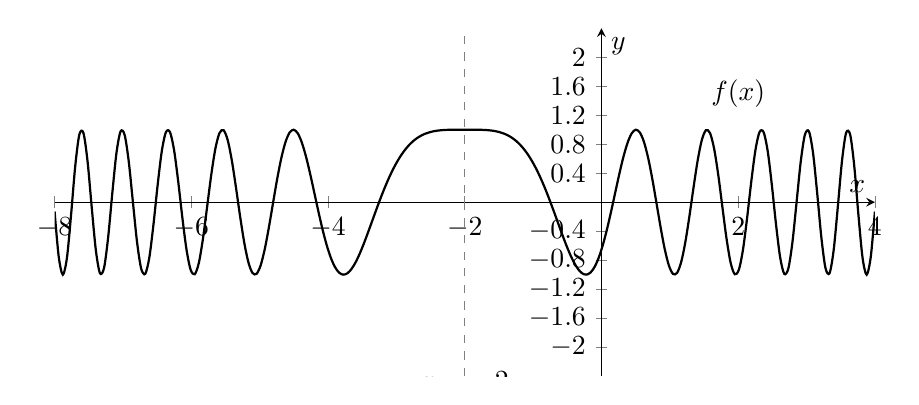
\begin{tikzpicture}
\begin{axis}[
 width=12cm,
 height=6cm,
 xlabel={$x$},
 ylabel={$y$},
 xmin=-8, xmax=4,
 ymin=-2.4, ymax=2.4,
 axis lines=middle,
 samples=200,
 ytick={-2,-1.6,-1.2,-0.8,-0.4,0,0.4,0.8,1.2,1.6,2},
]

% Plot f(x) = cos(x^2 + 4x + 4)
\addplot[thick, black, smooth, domain=-8:4] {cos(deg((x+2)^2))};
\node at (axis cs:2,1.5) {$f(x)$};

% Mark axis of symmetry
\addplot[dashed, gray] coordinates {(-2,-2.4) (-2,2.4)};
\node at (axis cs:-2,-2.2) [below] {$x = -2$};

\end{axis}
\end{tikzpicture}
\end{center}

\textbf{(a)} State the equation of the axis of symmetry of $f$. \hfill [1 mark]

\vspace{9\baselineskip}

\textbf{(b)} The graph of $f$ is mapped onto the graph of $y = \cos(x^2 + 2ax + a)$, where $a \in \mathbb{R}$, by a translation of $k$ units in the positive $x$-direction. Find the value(s) of $k$. \hfill [2 marks]

\vspace{9\baselineskip}

\hrulefill

\section*{Question 34 [TF]}

\textbf{Part (e)} \hfill 1 mark

Consider the function $g : [m,n] \to \mathbb{R}$, $g(x) = e^{\cos(x)} - 2$, where $m, n \in \mathbb{Z}$ and $m < n$.

As $m$ ranges over its domain, what is the maximum number of integers $n$ for which $g$ has an inverse?

\vspace{9\baselineskip}

\hrulefill

\section*{Question 35 [TA]}

\textbf{Part (f)}

Let $g : \mathbb{R} \to \mathbb{R}$, $g(x) = x^4 - 4x^3 + 2x^2(a-3) + 4x(a+1)$, where $a \in \mathbb{R}$.

Find all solutions to $g'(x) = 0$. Express your answer in terms of $a$.

\vspace{9\baselineskip}

\hrulefill

\section*{Question 36 [TA]}

\textbf{Part (iii)}

Find the values of $a$ for which the graph of $g$ has an absolute minimum in the fourth quadrant.

\vspace{9\baselineskip}

\hrulefill

\section*{Question 37 [TA]}

Let $h : [0,\infty) \to \mathbb{R}$, $h(x) = \frac{x^3 + k^2x}{20}$, where $k \geq 0$.

The graphs of $h$ and its inverse function $h^{-1}$ have a bounded area between them.

\textbf{(d)} Find the set of values of $k$ for which the graphs of $h$ and its inverse function $h^{-1}$ have a bounded area. \hfill [1 mark]

\vspace{9\baselineskip}

\textbf{(e)} Find the maximum area bounded by the graphs of $h$ and $h^{-1}$. \hfill [2 marks]

\vspace{9\baselineskip}

\textbf{(f)} Find the value of $k$ for which the line $y = 2 - x$ bisects the area bounded by the graphs of $h$ and $h^{-1}$. Give your answer correct to three decimal places. \hfill [3 marks]

\vspace{9\baselineskip}

\hrulefill

\section*{Question 38 [TF]}

\textbf{Question 8} \hfill 7 marks

Let $f : \mathbb{R} \to \mathbb{R}$, $f(x) = \log_e(x-k)$, where $k \in \mathbb{R}^+$, and $f^{-1}$ be the inverse function of $f$. The graphs of $y = f(x)$ and $y = f^{-1}(x)$ are shown below.

\begin{center}
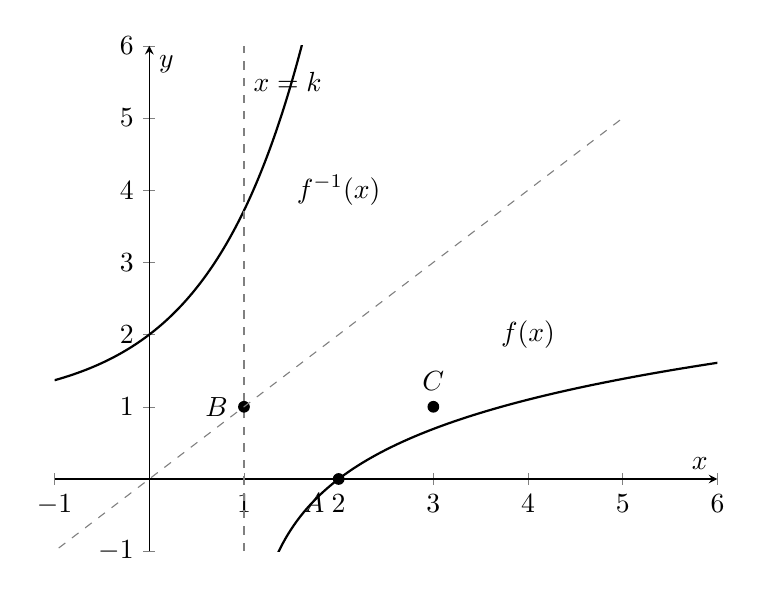
\begin{tikzpicture}
\begin{axis}[
 width=10cm,
 height=8cm,
 xlabel={$x$},
 ylabel={$y$},
 xmin=-1, xmax=6,
 ymin=-1, ymax=6,
 axis lines=middle,
 samples=100,
]

% Plot f(x) = ln(x-k) where k is shown as vertical asymptote
\addplot[thick, black, smooth, domain=1.1:6] {ln(x-1)};
\node at (axis cs:4,2) {$f(x)$};

% Plot f^{-1}(x) = e^x + k
\addplot[thick, black, smooth, domain=-1:2] {exp(x)+1};
\node at (axis cs:2,4) {$f^{-1}(x)$};

% Vertical asymptote x = k
\addplot[dashed, gray] coordinates {(1,-1) (1,6)};
\node at (axis cs:1,5.5) [right] {$x = k$};

% Points A, B, C
\node[circle,fill,inner sep=1.5pt, label=below left:$A$] at (axis cs:2,0) {};
\node[circle,fill,inner sep=1.5pt, label=left:$B$] at (axis cs:1,1) {};
\node[circle,fill,inner sep=1.5pt, label=above:$C$] at (axis cs:3,1) {};

% Line y = x
\addplot[dashed, gray] {x};

\end{axis}
\end{tikzpicture}
\end{center}

Point $A$ is the $x$-intercept of $f$ and point $B$ is the $y$-intercept of $f^{-1}$. The horizontal line through $B$ intersects the graph of $f$ at point $C$.

\textbf{(c)} The area of the region bounded by the $x$-axis, the line $x = k$, the horizontal line through point $B$, and the graph of $f$ is 2 square units. Find the value of $k$. Express your answer in the form $\log_e(a) + b$, where $a, b \in \mathbb{Z}$. \hfill [2 marks]

\vspace{9\baselineskip}

\hrulefill

\section*{Question 39 [TA]}

\textbf{Question 13} \hfill 1 mark

For a sample proportion $p$, what is the effect on the width of the 95\% confidence interval if the sample size is increased by a factor of 3?

\begin{enumerate}
    \item[A.] Increase by 73.2\%
    \item[B.] Decrease by 66.7\%
    \item[C.] Decrease by 33.3\%
    \item[D.] Decrease by 57.7\%
    \item[E.] Decrease by 42.3\%.
\end{enumerate}

\vspace{9\baselineskip}

\hrulefill

\section*{Question 40 [TA]}

\textbf{Part (d)} \hfill 3 marks

The weights of patients who take the drug are normally distributed with an interquartile range of 8 kilograms.

Find the standard deviation of the weights of patients. Give your answer in kilograms, correct to two decimal places.

Note: The interquartile range is defined as the difference between the 75th percentile and 25th percentile.

\vspace{9\baselineskip}

\hrulefill

\section*{Question 41 [TA]}

\textbf{Question 3} \hfill 11 marks

A river valley is modelled by the function $h : [0,12] \to \mathbb{R}$, $h(x) = 3\sin\left(\frac{\pi x}{4}\right) - \cos\left(\frac{\pi x}{2}\right) + 1$, where $h(x)$ decametres is the height of a point above the river surface ($y = 0$).

In the figure below, sections $AC$ and $DB$ represent the hills on the valley and $CD$ represents the river.

\begin{center}
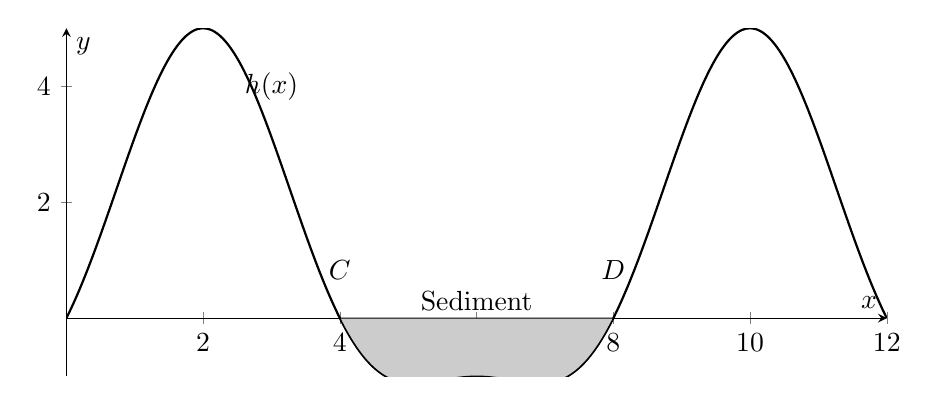
\begin{tikzpicture}
\begin{axis}[
 width=12cm,
 height=6cm,
 xlabel={$x$},
 ylabel={$y$},
 xmin=0, xmax=12,
 ymin=-1, ymax=5,
 axis lines=middle,
 samples=200,
]

% Plot h(x) = 3sin(πx/4) - cos(πx/2) + 1
\addplot[thick, black, smooth, domain=0:12] {3*sin(deg(pi*x/4)) - cos(deg(pi*x/2)) + 1};
\node at (axis cs:3,4) {$h(x)$};

% Mark points A, C, D, B
\node at (axis cs:0,0) [below left] {$A$};
\node at (axis cs:4,0.5) [above] {$C$};
\node at (axis cs:8,0.5) [above] {$D$};
\node at (axis cs:12,0) [below right] {$B$};

% Shaded region for sediment
\addplot[fill=gray!40, domain=4:8] {3*sin(deg(pi*x/4)) - cos(deg(pi*x/2)) + 1} \closedcycle;
\node at (axis cs:6,0.3) {Sediment};

\end{axis}
\end{tikzpicture}
\end{center}

Note: 1 decametre (dam) is equal to 10 metres.

\textbf{(g)} Sediment deposits formed at the bottom of the river, with the top layer modelled as a horizontal line in the figure. If the area of the shaded region is 0.75 square decametres, find the depth of the top layer of sediment from the surface of the water, in decametres. Give your answer correct to two decimal places. \hfill [3 marks]

\vspace{9\baselineskip}

\textbf{(h)} The rate of increase of sediment height was monitored for five years. After the third year of monitoring, the increase in sediment height was found to be 5 millimetres, and after 5 years the total increase in height (from the start of monitoring) was 7.5 millimetres.

If the rate of increase in height can be modelled by the function $r(t) = ae^{-bt}$, where $r(t)$ millimetres per year is the rate of increase in height $t$ years after the start of monitoring and $a, b \in \mathbb{R}^+$, find the values of $a$ and $b$. Give your answer correct to four decimal places. \hfill [2 marks]

\vspace{9\baselineskip}

\hrulefill

\section*{Question 42 [TA]}

\textbf{Question 4} \hfill 13 marks

Let $f : D \to \mathbb{R}$, $f(x) = \log_e((x-1)(x+3))$, where $D$ is the maximal domain of $f$. The graph of $y = f(x)$ is shown below.

\begin{center}
\begin{tikzpicture}
\begin{axis}[
 width=12cm,
 height=8cm,
 xlabel={$x$},
 ylabel={$y$},
 xmin=-10, xmax=10,
 ymin=-4, ymax=6,
 axis lines=middle,
 samples=200,
]

% Plot f(x) = ln((x-1)(x+3))
\addplot[thick, black, smooth, domain=-10:-3.1] {ln(abs((x-1)*(x+3)))};
\addplot[thick, black, smooth, domain=1.1:10] {ln(abs((x-1)*(x+3)))};
\node at (axis cs:6,4) {$f(x)$};

% Vertical asymptotes
\addplot[dashed, gray] coordinates {(-3,-4) (-3,6)};
\addplot[dashed, gray] coordinates {(1,-4) (1,6)};

\end{axis}
\end{tikzpicture}
\end{center}

\textbf{iii.} Find the set of values of $x_0$ for which $x_1$ exists but $f(x_1)$ does not. Give values correct to one decimal place. \hfill [3 marks]

\vspace{9\baselineskip}

\hrulefill

\section*{Question 43 [TF]}

\textbf{Question 5} \hfill 4 marks

Let $A$ and $B$ be events in a sample space $S$ such that $\Pr(B \mid A) = \frac{1}{6}$, $\Pr(A \mid B) = \frac{1}{3}$ and $\Pr(A \cap B) = p$.

\textbf{(a)} Find $\Pr(A)$ and $\Pr(B)$ in terms of $p$.

\vspace{9\baselineskip}

\textbf{(b)} If $\Pr(A' \cup B') \geq \Pr(A \cup B)$, find the complete range of values $p$ can take.

\vspace{9\baselineskip}

\hrulefill

\section*{Question 44 [TA]}

\textbf{Question 5} \hfill 12 marks

Let $g : (-\infty, \log_e(3)] \to \mathbb{R}$, $g(x) = 3x - e^x$. In the figure below, point $Q(b,0)$ is the $x$-intercept of $g$ and point $P(a,g(a))$, where $a > b$, is a point on the graph of $y = g(x)$.

\begin{center}
\begin{tikzpicture}
\begin{axis}[
 width=10cm,
 height=7cm,
 xlabel={$x$},
 ylabel={$y$},
 xmin=-1, xmax=2,
 ymin=-3, ymax=2,
 axis lines=middle,
 samples=100,
]

% Plot g(x) = 3x - e^x
\addplot[thick, black, smooth, domain=-1:1.1] {3*x - exp(x)};
\node at (axis cs:0.5,1.5) {$g(x)$};

% Point Q(b,0) and P(a,g(a))
\node[circle,fill,inner sep=1.5pt, label=below:$Q(b,0)$] at (axis cs:0.619,0) {};
\node[circle,fill,inner sep=1.5pt, label=above:$P(a,g(a))$] at (axis cs:1,3-exp(1)) {};

\end{axis}
\end{tikzpicture}
\end{center}

\textbf{(c)} In the figure below, line $l$ is perpendicular to the line $y = x$. It intersects the graphs of $g$ and $g^{-1}$ at $P(a,g(a))$ and $P'$, respectively. Point $Q'$ is the $y$-intercept of $g^{-1}$.

\begin{center}
\begin{tikzpicture}
\begin{axis}[
 width=10cm,
 height=10cm,
 xlabel={$x$},
 ylabel={$y$},
 xmin=-3, xmax=2,
 ymin=-3, ymax=2,
 axis lines=middle,
 samples=100,
]

% Plot g(x) = 3x - e^x
\addplot[thick, black, smooth, domain=-1:1.1] {3*x - exp(x)};
\node at (axis cs:0.5,1.5) {$g(x)$};

% Plot g^(-1)(x) (reflection over y=x)
\addplot[thick, black, smooth, domain=-2:1] {x}; % placeholder for g^(-1)
\node at (axis cs:-2,-1.5) {$g^{-1}(x)$};

% Line y = x
\addplot[dashed, gray, domain=-3:2] {x};
\node at (axis cs:1.5,1.7) {$y = x$};

% Line l perpendicular to y=x
\addplot[thick, gray, domain=-2:2] {-x+1};
\node at (axis cs:1,-0.5) {$l$};

% Points
\node[circle,fill,inner sep=1.5pt, label=above:$P(a,g(a))$] at (axis cs:1,3-exp(1)) {};
\node[circle,fill,inner sep=1.5pt, label=right:$P'$] at (axis cs:3-exp(1),1) {};
\node[circle,fill,inner sep=1.5pt, label=left:$Q'$] at (axis cs:0,0.619) {};
\node[circle,fill,inner sep=1.5pt, label=below:$O$] at (axis cs:0,0) {};
\node[circle,fill,inner sep=1.5pt, label=below:$Q(b,0)$] at (axis cs:0.619,0) {};

\end{axis}
\end{tikzpicture}
\end{center}

\textbf{iii.} There is a value of $a$ for which the area bounded by the graphs of $g$, $g^{-1}$, $l$ and the coordinate axes is equal to 0.5. Find this value, correct to two decimal places. \hfill [2 marks]

\vspace{9\baselineskip}

\hrulefill

\section*{Question 45 [TA]}

\textbf{Part (d)} \hfill 3 marks

Let $h : (-\infty, \log_e(k)] \to \mathbb{R}$, $h(x) = kx - e^x$, where $k > 0$, and $h^{-1}(x)$ be the inverse function of $h$.

If $h(c) = h^{-1}(c)$, find the maximum value of $c$ and the value of $k$ for which this occurs. Give your answers correct to two decimal places.

\vspace{9\baselineskip}

\hrulefill

\section*{Question 46 [TF]}

\textbf{Question 9}

Let $f : \mathbb{R} \to \mathbb{R}$, $f(x) = 2x^2 + 6x$.

\textbf{(c)} The graphs of $y = f(x - a) + b$ and $y = 2x$, where $a, b \in \mathbb{R}$, intersect at exactly one point. Find the values of $a$ and $b$ for which the quantity $a^2 + b^2$ is minimised. \hfill [4 marks]

\vspace{9\baselineskip}

\textbf{(b)} Find the set of values of $k$, where $k \in \mathbb{R}$, for which there is no tangent to the graph of $y = f(x - k)$ that passes through the point $(2,0)$. \hfill [1 mark]

\vspace{9\baselineskip}

\hrulefill

\section*{Question 47 [TA]}

\textbf{Question 16}

Let $f : \mathbb{R} \setminus \left\{\frac{a}{4}\right\} \to \mathbb{R}$, $f(x) = \frac{2}{4x-a} + 3$, where $a$ is a real constant.

Newton's method, with an initial estimate $x_0$, will fail when finding the root for the function $f$, if

\begin{enumerate}
    \item[A.] $x_0 \in \mathbb{R} \setminus \left[\frac{3a-4}{12}, \frac{a}{4}\right)$ only
    \item[B.] $x_0 = \frac{a}{4}$ only
    \item[C.] $\frac{3a-4}{12} \leq x_0 < \frac{a}{4}$
    \item[D.] $x_0 \in \mathbb{R} \setminus \left(\frac{3a-4}{12}, \frac{a}{4}\right)$
\end{enumerate}

\vspace{9\baselineskip}

\hrulefill

\section*{Question 48 [TA]}

\textbf{Question 2} \hfill 15 marks

A tidal river, at a particular station, Station A, has its height above ground level modelled by the function
\[
h_A(t) = a\sin(b(t-18)) + c
\]
for some $a, b, c \in \mathbb{R}^+$, with height, $h_A$, in metres $t$ hours after 9 am on a particular day.

On this day the river had a maximum height of 50 metres and minimum height of 10 metres.

\textbf{a.} Explain why $a = 20$ and $c = 30$. \hfill 1 mark

\vspace{9\baselineskip}

One complete cycle of the height, $h$, of the tidal river is completed in 18 hours.

\textbf{b.} Show that $b = \frac{\pi}{9}$. \hfill 1 mark

\vspace{9\baselineskip}

After 27 hours the tidal height at \textbf{Station A} changes, and from 9 am is modelled by the piecewise function $w$, defined by
\[
w(t) = \begin{cases}
h_A(t) & 0 \leq t \leq 27 \\
30 & 27 < t \leq 40
\end{cases}
\]

After 40 hours the tidal height changes again and the height, $p$ metres, at time $t$ hours after 9 am on a Sunday of a certain week can be modelled by the function
\[
p(t) = \begin{cases}
w(t) & 0 \leq t \leq 40 \\
m\cos(n(t-r)) + s & 40 < t \leq k
\end{cases}
\]
where $m$, $n$, $r$, $s$ and $k$ are real constants.

Recording capacities for this river break down at 9 pm on Tuesday of that particular week and no records of height are taken after this time.

\textbf{h.} State the value of $k$. \hfill 1 mark

\vspace{9\baselineskip}

The graph of $p(t)$ is continuous and smooth at $t = 40$ with the section described by $p = m\cos(n(t-r)) + s$ completing two cycles before recording capacities break.

Surprisingly for the recorders, the river over the domain $t \in [0,k]$ reaches zero height twice.

\textbf{i.} State a possible set of values for $m$, $n$, and $s$ and give $r$ as a general solution for those values. \hfill 3 marks

\vspace{9\baselineskip}

\hrulefill

\section*{Question 49 [TF]}

\textbf{Question 7} \hfill 4 marks

Consider the function $f$ with rule $f(x) = x + \frac{1}{x-2}$. Part of the graph of $f$ is shown below.

\begin{center}
\begin{tikzpicture}
\begin{axis}[
 width=10cm,
 height=8cm,
 xlabel={$x$},
 ylabel={$y$},
 xmin=-2, xmax=6,
 ymin=-6, ymax=6,
 axis lines=middle,
 samples=100,
]

% Plot f(x) = x + 1/(x-2)
\addplot[thick, black, smooth, domain=-2:1.85] {x + 1/(x-2)};
\addplot[thick, black, smooth, domain=2.15:6] {x + 1/(x-2)};

% Vertical asymptote x = 2
\addplot[dashed, gray] coordinates {(2,-6) (2,6)};

% Mark origin
\node at (axis cs:0,0) [below left] {$O$};

\end{axis}
\end{tikzpicture}
\end{center}

\textbf{ii.} Find the value of $a$, where $a \in R$, for which the graph of $y = 1 + f(a-x)$ has no $y$-intercepts. \hfill 1 mark

\vspace{9\baselineskip}

\hrulefill

\section*{Question 50 [TF]}

\textbf{Question 9} \hfill 8 marks

The diagram below shows a trapezium with vertices at $(0,0)$, $(0,2)$, $(3,2)$ and $(b,0)$, where $b$ is a real number and $0 < b < 2$.

\begin{center}
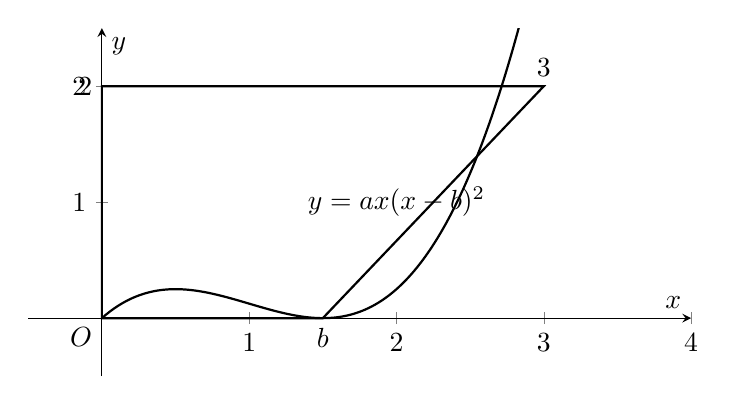
\begin{tikzpicture}
\begin{axis}[
 width=10cm,
 height=6cm,
 xlabel={$x$},
 ylabel={$y$},
 xmin=-0.5, xmax=4,
 ymin=-0.5, ymax=2.5,
 axis lines=middle,
 samples=100,
]

% Trapezium
\draw[thick] (axis cs:0,0) -- (axis cs:0,2) -- (axis cs:3,2) -- (axis cs:1.5,0) -- cycle;

% Cubic curve
\addplot[thick, black, smooth, domain=0:3] {x*(x-1.5)^2/2};
\node at (axis cs:2,1) {$y = ax(x-b)^2$};

% Label points
\node at (axis cs:0,0) [below left] {$O$};
\node at (axis cs:0,2) [left] {$2$};
\node at (axis cs:3,2) [above] {$3$};
\node at (axis cs:1.5,0) [below] {$b$};

\end{axis}
\end{tikzpicture}
\end{center}

On the same axes as the trapezium, part of the graph of a cubic polynomial function is drawn. It has the rule $y = ax(x-b)^2$, where $a$ is a non-zero real number and $0 \leq x \leq b$.

\textbf{a.} At the local maximum of the graph, $y = b$.

Find $a$ in terms of $b$. \hfill 3 marks

\vspace{9\baselineskip}

\hrulefill

\section*{Question 51 [TF]}

\textbf{Question 7} \hfill 9 marks

Let $f : \left[0, \frac{\pi}{2}\right] \to R$, $f(x) = 4\cos(x)$ and $g : \left[0, \frac{\pi}{2}\right] \to R$, $g(x) = 3\sin(x)$.

\textbf{b.} Let $c$ be such that $f(c) = g(c)$, where $c \in \left[0, \frac{\pi}{2}\right]$.

Find the value of $\sin(c)$ and the value of $\cos(c)$.

\vspace{9\baselineskip}

\hrulefill

\section*{Question 52 [TA]}

\textbf{Question 17}

If $F(x)$ is an antiderivative of $f(x)$ and $F(4) = -6$, then $F(8)$ is equal to

\begin{enumerate}
    \item[A.] $f'(8) + 6$
    \item[B.] $-6 + f'(4)$
    \item[C.] $\int_4^8 f(x)\,dx$
    \item[D.] $\int_4^8 (-6 + f(x))\,dx$
    \item[E.] $-6 + \int_4^8 f(x)\,dx$
\end{enumerate}

\vspace{9\baselineskip}

\hrulefill

\section*{Question 53 [TA]}

\textbf{Part f} \hfill 2 marks

A knob is attached to each controller. The height of a knob is normally distributed with a mean of 30 mm. If the knob on a controller has a height greater than 30.4 mm or less than 29.6 mm, then the controller is defective.

Rebecca wants to ensure that less than 2\% of all controllers manufactured are defective.

What is the maximum standard deviation of the height of a knob, in millimetres, that can be attached to a controller so that less than 2\% of controllers are defective? Give your answer correct to two decimal places.

\vspace{9\baselineskip}

\hrulefill

\section*{Question 54 [TF]}

\textbf{Question 7} \hfill 8 marks

The shaded region in the diagram below is bounded by the vertical axis, the graph of the function with rule $f(x) = \sin(\pi x)$ and the horizontal line segment that meets the graph at $x = a$, where $1 \leq a \leq \frac{3}{2}$.

\begin{center}
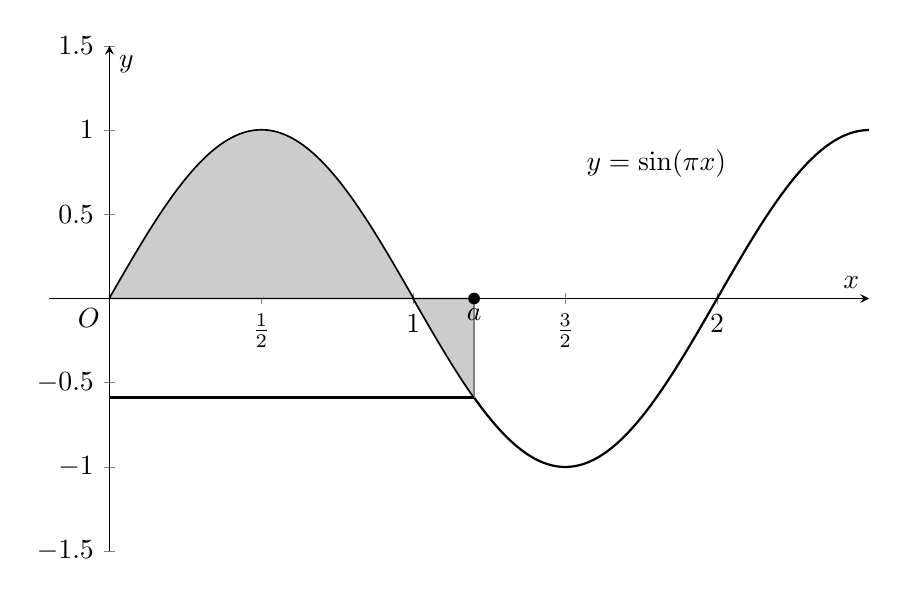
\begin{tikzpicture}
\begin{axis}[
 width=12cm,
 height=8cm,
 xlabel={$x$},
 ylabel={$y$},
 xmin=-0.2, xmax=2.5,
 ymin=-1.5, ymax=1.5,
 axis lines=middle,
 samples=200,
 xtick={0,0.5,1,1.5,2},
 xticklabels={$0$,$\frac{1}{2}$,$1$,$\frac{3}{2}$,$2$},
]

% Plot y = sin(πx)
\addplot[thick, black, smooth, domain=0:2.5] {sin(deg(pi*x))};
\node at (axis cs:1.8,0.8) {$y = \sin(\pi x)$};

% Shaded region (example with a = 1.2)
\addplot[fill=gray!40, domain=0:1.2] {sin(deg(pi*x))} \closedcycle;
\addplot[thick, gray, domain=0:1.5] coordinates {(1.2,{sin(deg(pi*1.2))}) (1.2,0)};
\draw[thick] (axis cs:0,{sin(deg(pi*1.2))}) -- (axis cs:1.2,{sin(deg(pi*1.2))});

% Mark point a
\node[circle,fill,inner sep=1.5pt] at (axis cs:1.2,0) {};
\node at (axis cs:1.2,0) [below] {$a$};

% Mark origin
\node at (axis cs:0,0) [below left] {$O$};

\end{axis}
\end{tikzpicture}
\end{center}

Let $A(a)$ be the area of the shaded region.

\textbf{a.} Show that $A(a) = \frac{1}{\pi} - \frac{1}{\pi}\cos(a\pi) - a\sin(a\pi)$. \hfill 3 marks

\vspace{9\baselineskip}

\textbf{c. i.} Express in terms of $A(a)$, for a specific value of $a$, the area bounded by the vertical axis, the graph of $y = 2\left(\sin(\pi x) + \frac{\sqrt{3}}{2}\right)$ and the horizontal axis. \hfill 2 marks

\vspace{9\baselineskip}

\textbf{ii.} Hence, or otherwise, find the area described in \textbf{part c.i.}

\vspace{9\baselineskip}

\hrulefill

\section*{Question 55 [TF]}

\textbf{Question 8} \hfill 5 marks

A fair standard die is rolled 50 times. Let $W$ be a random variable with binomial distribution that represents the number of times the face with a six on it appears uppermost.

\textbf{a.} Write down the expression for $\Pr(W = k)$, where $k \in \{0, 1, 2, \ldots, 50\}$. \hfill 1 mark

\vspace{9\baselineskip}

\textbf{b.} Show that $\frac{\Pr(W = k+1)}{\Pr(W = k)} = \frac{(50-k)}{5(k+1)}$. \hfill 2 marks

\vspace{9\baselineskip}

\textbf{c.} Hence, or otherwise, find the value of $k$ for which $\Pr(W = k)$ is the greatest. \hfill 2 marks

\vspace{9\baselineskip}

\hrulefill

\section*{Question 56 [TA]}

\textbf{Question 9}

At the start of a particular week, Kim has three red apples and two green apples. She eats one apple every day. On Monday, Tuesday and Wednesday of that week, she randomly selects an apple to eat.

In this three-day period, the probability that Kim does not eat an apple of the same colour on any two consecutive days is

\begin{enumerate}
    \item[A.] $\frac{1}{10}$
    \item[B.] $\frac{1}{5}$
    \item[C.] $\frac{3}{10}$
    \item[D.] $\frac{2}{5}$
    \item[E.] $\frac{6}{25}$
\end{enumerate}

\vspace{9\baselineskip}

\end{document}
